\part{Polarisation circulaire, molécules chirales et harmoniques d'ordre élevé}
\label{PA:Spin_HHG}
\chapter{Génération d'harmoniques d'ordre élevé polarisée elliptiquement}
\label{CH:Circular_HHG}
Dans cette partie nous présenterons comment générer des harmoniques d'ordre élevé portant du moment angulaire de spin, c'est-à-dire ayant une polarisation elliptique. Nous présenterons pour commencer le formalisme utile à la description d'ondes polarisées, puis étudierons le mécanisme de GHOE dans un atome quand le laser de génération est polarisé elliptiquement. Nous verrons que ce mécanisme présente des difficultés intrinsèques et mentionnerons les solutions existantes, avant d'en démontrer une nouvelle qui utilise une résonance de l'atome ou la molécule de génération.

\section{Formalisme pour la description d'ondes polarisées elliptiquement}
Comme on l'a vu dans la partie \ref{sec:circpolar}, le champ électrique d'une onde polarisée elliptiquement décrit une ellipse au cours de sa propagation. Soit $(x,y,z)$ un repère cartésien tel que $z$ soit selon la direction de propagation et $x$ selon l'axe majeur de l'ellipse. Le champ, que l'on considère monochromatique, s'écrit :
\begin{equation}
\bm{E}=\begin{pmatrix}
E_{x}\cos{(\omega t-kz)}\\
E_{y}\sin{(\omega t-kz)}\\
0
\end{pmatrix}=E_{0}
\begin{pmatrix}
\cos{(\omega t-kz)}\\
\epsilon\sin{(\omega t-kz)}\\
0
\end{pmatrix},
\label{eq:jones}
\end{equation}
où $\epsilon = E_{y}/E_{x}$ est appelé ellipticité du champ. $\epsilon$ varie de 0 pour une polarisation linéaire à 1 pour une polarisation circulaire.  On a vu que si $\epsilon>0$ (resp. $<0$), l'onde était elliptique gauche (resp. droite) et porte un moment angulaire de spin de $\hbar$ (resp. $-\hbar$). 

\begin{figure}[!ht]
\centering
\def\svgwidth{0.6\columnwidth}
\import{Figures/Polar/}{polarellipse.pdf_tex}
\caption{Définition des différents paramètres de l'ellipse de polarisation.}
\label{Fig:polarellipse}
\end{figure}
Dans un repère où $x$ et $y$ ne sont pas selon les axes de l'ellipse (voir figure \ref{Fig:polarellipse}), on note $\eta$ l'angle entre l'axe $x$ et l'axe majeur de l'ellipse. L'ellipticité est déterminée par le rapport des axes mineurs et majeurs de l'ellipse, $b$ et $a$ : $\epsilon = b/a$. On note $\chi$ l'angle tel que $\tan\chi = \epsilon = b/a$. Comme les amplitudes du champ selon les axes de l'ellipse sont déphasées de $\pi/2$, $a$ et $b$ peuvent être vus comme les parties réelle et imaginaire d'un vecteur de polarisation complexe et unitaire $\bm{\Pi}$. Le champ s'écrit alors :
\[\bm{E} = E_x \bm{e_x} + E_y \bm{e_y} = E_0(\Pi_x \bm{e_x} + \Pi_y \bm{e_y}).\] 
Il sera utile d'utiliser les \textit{paramètres de Stokes}, définis comme :
\begin{align}
S_0 &= E_xE_x^*+E_yE_y^* =E_0^2,\nonumber\\
S_1 &= E_xE_x^*-E_yE_y^* =E_0^2\cos 2\chi\cos 2\eta ,\nonumber\\
S_2 &= -\left(E_xE_y^*+E_yE_x^*\right)=E_0^2\cos 2\chi\sin 2\eta,\nonumber\\
S_3 &= -\rmi\left(E_xE_y^*-E_yE_x^*\right)=E_0^2\sin 2\chi,	
\label{eq:stokes1}
\end{align}
où nous avons utilisés les conventions de signe de \mycite{barron}. Pour une onde monochromatique, ces paramètres donnent $E_0$, $\chi$ et $\eta$, ou de manière équivalente, l'intensité $I_0$, l'ellipticité $\epsilon$ et $\eta$. Ils caractérisent donc totalement le champ électrique. Il ne sont pas indépendants : on a $S_0^2 = S_1^2+S_2^2+S_3^2$. 

En pratique, les ondes utilisées ne sont que \textit{quasi}-monochromatiques. Elles possèdent une largeur spectrale $\Delta\omega$ non nulle, à l'intérieur de laquelle les différentes composantes fréquentielles ne possèdent pas forcément les mêmes polarisations et phases. Le vecteur du champ électrique apparent ne décrit alors plus une ellipse. Dans le cas extrême, il ne présente aucune direction préférentielle : on parle alors de lumière \textit{non polarisée}. De manière générale, le vecteur du champ électrique n'évolue pas complètement régulièrement ou irrégulièrement, la lumière est alors dite \textit{partiellement} polarisée.

Dans une expérience, le temps d'observation est en général long comparé à $1/\Delta\omega$. Les vecteurs de Stokes doivent donc être définis à partir de la moyenne temporelle des quantités définies en \ref{eq:stokes1}. Ces expressions font intervenir les produits des composantes de $\bm{\Pi}$. Pour une lumière complètement polarisée,
\[\overline{\Pi_x \Pi^*_y} = \Pi_x \Pi^*_y,\]
et on retrouve les mêmes propriétés que pour une onde monochromatique. \`{A} l'autre extrême, si la lumière est non polarisée, toutes les orientations de $\bm{\Pi}$ sont équiprobables :
\[\overline{\Pi_x \Pi^*_y} = 0.\]
Les paramètres de Stokes deviennent donc $S_0 = E_0^2$ et $S_1^2 = S_2^2 = S_3^2 = 0$. Dans le cas d'une lumière partiellement polarisée, on obtient donc $S_0^2 > S_1^2+S_2^2+S_3^2$. On introduit alors le degré de polarisation de la lumière $P$, défini comme 
\[P = \frac{\sqrt{S_1^2+S_2^2+S_3^2}}{S_0}.\] $P$ varie entre $0$ pour une lumière non polarisée et $1$ pour une polarisation complète. Une lumière partiellement polarisée peut être séparée entre une composante non polarisée et une complètement polarisée, dont les paramètres d'ellipse sont bien définis. On les retrouve à partir des paramètres de Stokes :
\begin{align}
S_0 &= E_0^2,\nonumber\\
S_1 &= PE_0^2\cos 2\chi\cos 2\eta ,\nonumber\\
S_2 &= PE_0^2\cos 2\chi\sin 2\eta,\nonumber\\
S_3 &= PE_0^2\sin 2\chi,	
\label{eq:stokes2}
\end{align}
L'onde est maintenant complètement décrite par $E_0$, $\chi$, $\eta$ et $P$. Cette description est similaire à celle d'un système en mécanique quantique. En effet, une description vectorielle telle que l'expression \ref{eq:jones} (appelé vecteur de Jones) est analogue à la fonction d'onde d'un système quantique. Elle ne peut décrire qu'une polarisation complète, analogue à un état quantique pur. Une polarisation partielle est une superposition incohérente de polarisations complètes, de même qu'un état quantique mixte est une superposition d'état purs. Pour les décrire, on fait appel au formalisme de Stokes pour la polarisation, et à la matrice densité pour un système quantique. Cette analogie n'est pas fortuite : la lumière provient généralement d'une transition entre deux états quantiques, par exemple d'un atome. Les propriétés de polarisation de la lumière découlent alors de la cohérence entre ces états, comme décrit par \mycite{fano1957}. 

Pour terminer, notons que la polarisation partielle de la lumière peut également découler d'une inhomogénéité spatiale : si les paramètres de l'ellipse varient avec la coordonnée transverse et que l'expérience moyenne spatialement ces différentes contributions, on aura $P<1$.

\section{GHOE à partir d'un faisceau infrarouge polarisé elliptiquement}
Dans la partie précédente, nous avons démontré qu'en donnant du moment angulaire orbital à l'infrarouge de génération, il était transmis au rayonnement harmonique. Ce principe devrait s'appliquer au moment angulaire de spin, qui doit être conservé dans le processus. 

\subsection{Résultats de la littérature}
\mycite{budilPRA1993} ont réalisé la première expérience à ce sujet. Ils ont généré les harmoniques d'ordre élevé d'un laser Cr:LiSAF et mesuré l'intensité de chaque harmonique en fonction de l'ellipticité de l'infrarouge. Le résultat pour le néon est présenté sur la figure \ref{Fig:budil}
\begin{figure}[!ht]
\centering
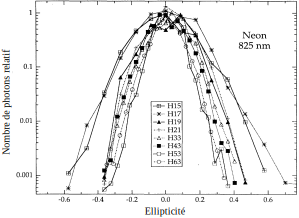
\includegraphics[width=0.6\columnwidth]{Figures/Polar/Intensity_f_ellipticity_budil}%
\caption{Intensité normalisée des harmoniques produites dans le néon en fonction de l'ellipticité. Tiré de \mycite{budilPRA1993}}%
\label{Fig:budil}%
\end{figure}
On observe une décroissance de l'intensité harmonique en fonction de l'ellipticité. Cet effet est marqué : on perd environ un ordre de grandeur en intensité quand $|\epsilon_{IR}| = 0.2$. On remarque également que cette décroissance est de plus en plus piquée lorsque l'ordre harmonique augmente.

\'{E}tudions ensuite les résultats de \mycite{AntoinePRA1997}. Les auteurs se sont cette fois intéressés à l'état de polarisation du rayonnement harmonique en fonction de l'ellipticité de l'infrarouge. Ces expériences ont été réalisées sur une version antérieure du système laser que nous avons utilisé dans la partie III. Pour caractériser le rayonnement, les auteurs mesurent des \textit{lois de Malus}, méthode optique qui sera présentée plus loin (section \ref{sec:malus}). Comme on le verra, cette technique est incapable de mesurer le degré de polarisation $P$. Elle ne donne qu'une borne supérieure sur l'ellipticité, atteinte uniquement lorsque la lumière est complètement polarisée. Ce point est crucial dans le cas de la GHOE : comme expliqué dans la partie \ref{sec:introHHG}, le dipôle de chaque ordre harmonique dépend de l'intensité infrarouge. Le champ émis sera donc non homogène en polarisation spatialement et temporellement, donc nécessairement partiellement polarisé.

La figure \ref{fig:antoinepra} présente quelques résultats extraits de \mycite{AntoinePRA1997}. On y voit l'évolution de l'ellipticité des harmoniques, $\epsilon_q$, et de l'angle d'orientation de l'ellipse par rapport à un axe de référence fixe, $\eta$. Comme expliqué, l'ellipticité mesurée n'est pas la véritable valeur. Pour en avoir une idée, la figure \ref{fig:antoinepra} inclut un résultat numérique qui donne accès à $P$.

\begin{figure}[!ht]
\centering
\def\svgwidth{\columnwidth}
\import{Figures/Polar/}{antoinePRA.pdf_tex}
\caption{\`{A} gauche, mesure de l'ellipticité des harmoniques 17 et 23 générées dans l'argon par un champ infrarouge elliptique. Carrés rouges : mesures expérimentales de $\epsilon_q$ par loi de Malus. Comme expliqué plus haut, ce n'est qu'une borne supérieure sur la vraie valeur de l'ellipticité. En traits rouges, même quantité obtenue par le calcul. En pointillés noirs, véritable ellipticité obtenue par le calcul. En traits-pointillés verts, degré de polarisation obtenu par le calcul. \`{A} droite, mesure de l'angle de rotation de l'ellipse (carrés rouges) et même quantité obtenue par le calcul (traits rouges). Adapté de \mycite{AntoinePRA1997}.}
\label{fig:antoinepra}
\end{figure}

On fait les observations suivantes :
\begin{itemize}
\renewcommand{\labelitemi}{$\bullet$}
\setlength\itemsep{1em}
\item $\epsilon_q$ est une fonction croissante de $\epsilon_{IR}$ sur l'intervalle parcouru.
\item $|\epsilon_q|$ augmente plus rapidement avec $|\epsilon_{IR}|$ pour l'harmonique plus basse.
\item Le rayonnement est de moins en moins polarisé à mesure que $|\epsilon_{IR}|$ augmente. Cet effet est plus fort pour l'harmonique basse.
\item Cette diminution de $P$ s'accompagne d'une ellipticité vraie plus faible. Pour l'harmonique la plus basse, l'ellipticité vraie est presque \textit{deux fois inférieure} à l'ellipticité mesurée.
\item $\eta$ est également une fonction croissante de $\epsilon_{IR}$.
\item $\eta$ augmente plus rapidement pour l'harmonique basse.
\end{itemize}
\vspace{\baselineskip}
Ces deux travaux démontrent deux résultats généraux. En premier lieu, on voit que l'ellipticité de l'infrarouge est bien transférée au champ harmonique. Toutefois, l'ellipticité harmonique semble toujours rester inférieure à celle du laser générateur. Deuxièmement, le rendement harmonique décroît exponentiellement avec l'ellipticité de l'infrarouge. Nous concluons donc qu'il est très difficile d'obtenir un rayonnement ultraviolet d'ellipticité significative tout en gardant un niveau de signal suffisant. Dans la section suivante, nous expliquons les effets physiques à l'origine de ces propriétés.

\subsection{Modèle théorique simple de la GHOE en polarisation elliptique}

\section{Solutions existantes}
\section{Génération résonante}

\chapter{Polarisation circulaire et chiralité}
\section{Définitions de la chiralité}
\section{Dichroïsme circulaire et activité optique}
\section{Dichroïsme circulaire de photoélectron (PECD)}

\chapter{Mesures de PECD avec une source d'harmoniques d'ordre élevé}
\section{Mesures de PECD dans la fenchone}
\section{Caractérisation de l'état de polarisation des harmoniques par le PECD}

\chapter{Mesures chiroptiques à l'échelle femtoseconde}
\section{Le PECD en régime multiphotonique}
\section{Création et mesure résolue en temps de densités chirales}